Under the understanding that the reactions of interest follow a pseudo-first order model, we are only considering single collisions between the two reactants. To figure out the characteristic rate of the rate constant $k$, we want to model the interaction between the reactants, whether it be neutral-neutral, to ion-dipole. To do this, we consider adiabatic capture theory, a study of the long range potentials between particles to yield a reaction rate constant. A caveat is that the adiabatic capture theory is long ranged, only finding the rate at which a collision will occur, not necessarily when a reaction will happen. The probability of a reaction occurring requires modeling of short range interactions within the reaction complex. But understanding capture theory will yield the maximally allowed rate of reactions, if all collisions lead to a reaction.

\subsection{Rate Constant Derivation} \label{sec: ACT}
A general method of calculating the rate constant of two particles with a given potential, finding the collisional cross section, which is then averaged over a velocity distribution to find the rate constant.\cite{Zhang2017} Starting with the attractive potential, we find that it is a summation of interactions with coefficients $C_n$, where $n$ is the order of the interaction potential on the intermolecular distance $r$.

\begin{equation}
    V(r) = \sum_n -\frac{C_n}{r^n}
\end{equation}

We may write the effective potential in the center of mass frame as:

\begin{equation}
    V_{eff} = \frac{l^2}{2 \mu_R r^2} -V(r)\label{eq: veff}
\end{equation}

Where $\mu_R$ is the reduced mass of the two particles. If $n > 2$, we can derive the capture cross-section and rate constant as follows. First, we find the position $r_0$ corresponding to the maximum of the effective potential, which is the maximum of the centrifugal barrier.

\begin{align*}
    \frac{\partial V_{eff}(r_0)}{\partial r} & = 0 \\
    \therefore r_0 & = \left(\frac{n \mu_R C_n}{l^2}\right)^{1/n-2}
\end{align*}

Substituting $r_0$ back into equation $\ref{eq: veff}$, we find the maximal value of the effective potential:

\begin{equation}
    V_{eff}(r_0) = \left(\frac{l^2}{\mu_R}\right)^{\frac{n}{n-2}} \frac{n-2}{2n}(n C_n)^{-\frac{2}{n-2}}
\end{equation}

This then defines the energy necessary for a collision, for if $E_{col}$ exceeds $V_{eff}(r_0)$, the reactants will be able to surmount the centrifugal barrier and collide. Thus, we may define the maximum value for the angular momentum $l$ and the impact parameter $b$.

\begin{align*}
    l_{max} & = (\mu_R n)^{1/2}(C_n)^{1/n} \left(\frac{2 E_{col}}{n-2}\right)^{\frac{n-2}{2n}} \\
    b_{max} & = \frac{l_{max}}{\mu_R v}
\end{align*}

We can then define a collision cross section dependent on the collision energy:

\begin{align*}
    \sigma(E_{col}) & = \pi b^2_{max} \\
    & = \frac{\pi}{2} n \left(\frac{2}{n-2}\right)^{\frac{n-2}{2}} \left(\frac{C_n}{E_{col}}\right)^{\frac{2}{n}}
\end{align*}

Integrating the collision cross section with a Maxwell Boltzmann distribution yields a generalized rate constant as a function of temperature and $n$.

\begin{align}
    k(T) & = \int_0^{\infty} v f(v) \sigma(v) dv \label{eq: k int} \\
    & = \sqrt{\frac{2 \pi}{\mu_R}}n\left(\frac{2}{n-2}\right)^{\frac{n-2}{2}}C_n^{2/n}(k_B T)^{\frac{n-4}{2n}}\Gamma\left(2-\frac{2}{n}\right) \label{eq: k(T)}
\end{align}

For instance, we are interested in the ion-induced dipole interaction of order $n=4$.

\begin{align}
	C_4 & = \frac{\alpha q^2}{2} \nonumber \\
	k(T) & = 2\pi q \sqrt{\frac{\alpha}{\mu_R}} \label{eq: k langevin}
\end{align}

Where $\alpha$ is the polarizability of the neutral reactant, and $q$ is the monopole charge. The corresponding $k$ value in \cref{eq: k langevin} is known as the Langevin rate constant, which is famously temperature independent.

\subsection{Average Dipole Orientation (ADO)}

Unlike the Langevin interaction, the ion-dipole term has an angular term defined with respect to the inter-molecular axis. A few approximations are taken in the average dipole orientation theory pioneered and expanded on by Su and Bowers.\cite{Su1973, Su1973a} This can also be extrapolated to include quadrupole interactions.\cite{Su1975}

The Langevin term of the ion and ion-induced dipole interaction is as follows:

\begin{align}
	V_L(r)= &-\frac{\alpha q^2}{2r^4}
\end{align}

In the case of the ion-dipole interaction:

\begin{align}
	V_D(r, \theta) = & -\frac{q\mu_D}{r^2} \cos(\theta)
\end{align}

The method outlined in section \ref{sec: ACT} finds the rate constant by dealing with a two body problem only needing to consider the $r$ degree of freedom. The inclusion of the $\theta$ term complicates this, but to first order, we can parameterize $\theta$ as a function of $r$. What we want to achieve is to write down the potential as such:

\begin{align}
    V(r) & = -\frac{\alpha q^2}{2r^4} - \frac{q\mu_D}{r^2} \cos\left(\bar{\theta}(r)\right) \nonumber \\
    \bar{\theta} & = \dfrac{\int \theta P(\theta) d\theta}{\int P(\theta) d\theta} \label{eq: avg theta}
\end{align}

Where $P(\theta)$ is the probability of finding the dipole oriented with angle $\theta$. To determine the average orientation of the dipole, we consider the following cases:

\begin{enumerate}
	\item $P(\theta)$ is inversely proportional to the angular velocity:
	\begin{equation*}
		P(\theta) \propto 1/\dot{\theta}
	\end{equation*}
	\item An orientation has a probability weighted by the circumference of an angle:
	\begin{align*}
		C & = 2\pi l \sin(\theta) \\
		P(\theta) & \propto \sin(\theta)
	\end{align*}
\end{enumerate}

Combining these two effects:

\begin{align}
    P(\theta) & \propto \frac{\sin(\theta)}{\dot{\theta}} \label{eq: prob}
\end{align}

Any non-$\theta$ contribution in equation \ref{eq: prob} is eliminated when applied to equation \ref{eq: p theta}, allowing us to move forward without fully knowing $P(\theta)$. We can relate the angular velocity to the angular kinetic energy and the total energy in the system:

\begin{align}
    KE_{rot} & = \frac{1}{2}I\dot{\theta}^2 \nonumber \\
    E_{tot} & = KE_{rot} + V_D \label{eq: Etot}
\end{align}

Redefining equation \ref{eq: prob} with equation \ref{eq: Etot}, we find:

\begin{equation}
    P(\theta) \propto \frac{\sin(\theta)}{\sqrt{E_{rot}-V_D}} \label{eq: p theta}
\end{equation}

Combining equations \cref{eq: p theta,eq: avg theta} yields a total averaged dipole orientation.

\begin{equation}
    \bar{\theta} = \dfrac{\displaystyle \int\frac{\theta \sin(\theta)d\theta}{\sqrt{E_{rot}+q\mu_D/r^2 \cos(\theta)}}}{\displaystyle \int\frac{\sin(\theta)d\theta}{\sqrt{E_{rot}+q\mu_D/r^2 \cos(\theta)}}} \label{eq: avg theta int}
\end{equation}

From here, two situations arise:

\begin{enumerate}
	\item $E_{rot} = E_1 < \frac{q \mu_D}{r^2}$:
	There is not enough rotational energy to overcome the dipole locking. The solution is oscillatory, but $\theta$ has an $r$ dependent bound. We let the maximal capture angle that rotational energy $E_1$ allows be defined as $K$.

	\begin{equation*}
		E_1=-\frac{q \mu_D}{r^2}\cos(K)
	\end{equation*}

	When substituted into equation \ref{eq: avg theta int}, we find:

	\begin{equation}
	    \bar{\theta}_1 = \dfrac{\displaystyle\int_0^K \frac{\theta \sin(\theta) d \theta}{\sqrt{\cos(\theta) - \cos(K)}}}{\displaystyle\int_0^K \frac{\sin(\theta) d \theta}{\sqrt{\cos(\theta) - \cos(K)}}} \label{eq: theta1}
	\end{equation}

	After integration by infinite series, we yield a result of:

	\begin{align*}
	    \bar{\theta}_1 & = \frac{2 \sqrt{2}A}{\sqrt{1-\cos(K)}} \\
	    \text{where }A & \equiv \int_0^{\pi/2} \frac{a^2 \cos(\phi)^2 d\phi}{\sqrt{1-a^2 \sin(\phi)^2}} \\
	    a & \equiv \sin\left(\frac{K}{2}\right)
	\end{align*}

	\begin{figure}[H]
		\label{fig: theta1}
		\centering
		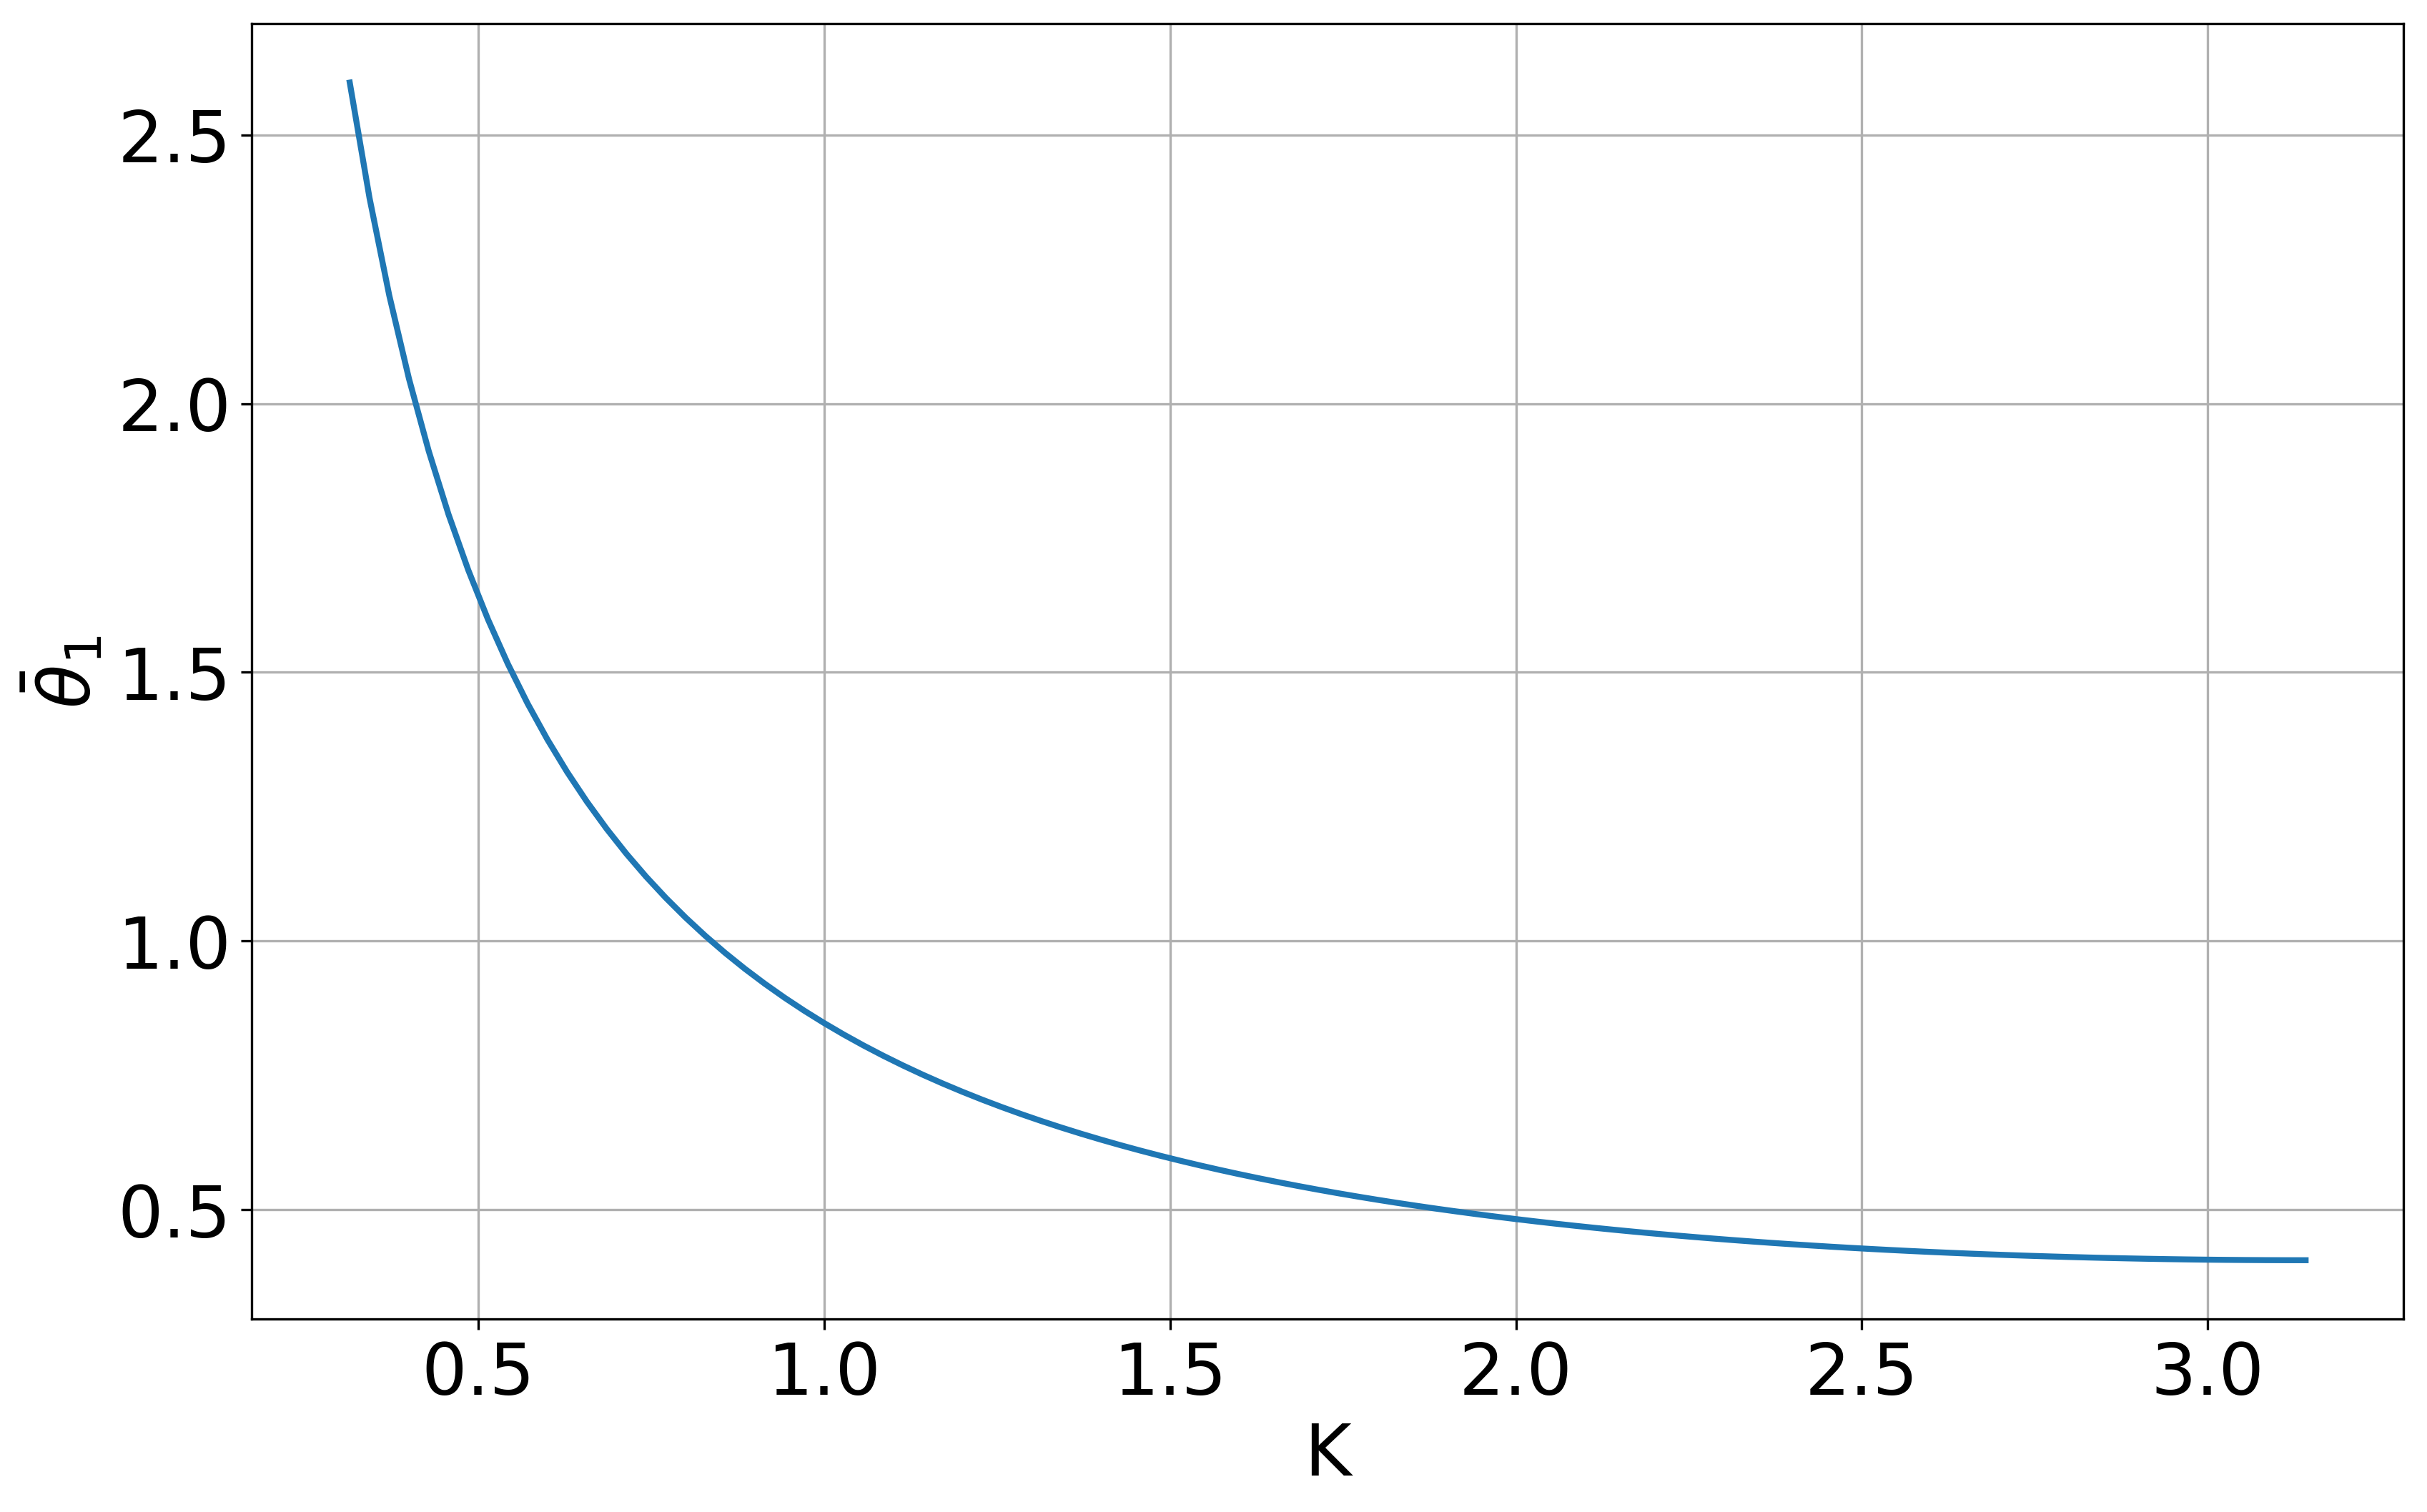
\includegraphics[width=0.8\textwidth]{images/ADO_theta1.png}
		\caption{Numerical solutions for reaction \ref{eq: theta1} as a function of maximum angle $K$. In the limit of large $K$, we find an intuitive solution where $\theta_1$ averages towards 0 where we have full dipole-locking.}
	\end{figure}

	\item $E_{rot} = E_2 > \frac{q \mu_D}{r^2}$:
	The rotational energy is enough to overcome the dipole locking and $\theta$ can swing around in a complete circle

	\begin{equation}
	    \bar{\theta}_2  = \dfrac{\displaystyle\int_0^\pi \frac{\theta \sin(\theta) d\theta}{\sqrt{E_2 + q \mu_D/r^2 \cos(\theta)}}}{\displaystyle\int_0^\pi \frac{\sin(\theta) d \theta}{\sqrt{E_2 + q \mu_D/r^2 \cos(\theta)}}} \label{eq: theta2}
	\end{equation}

	We no longer have bounds on the angles the dipole is allowed over, but the behavior is still dependent on the strength of the internal energy and dipole force.

	\begin{figure}[H]
		\label{fig: theta2}
		\centering
		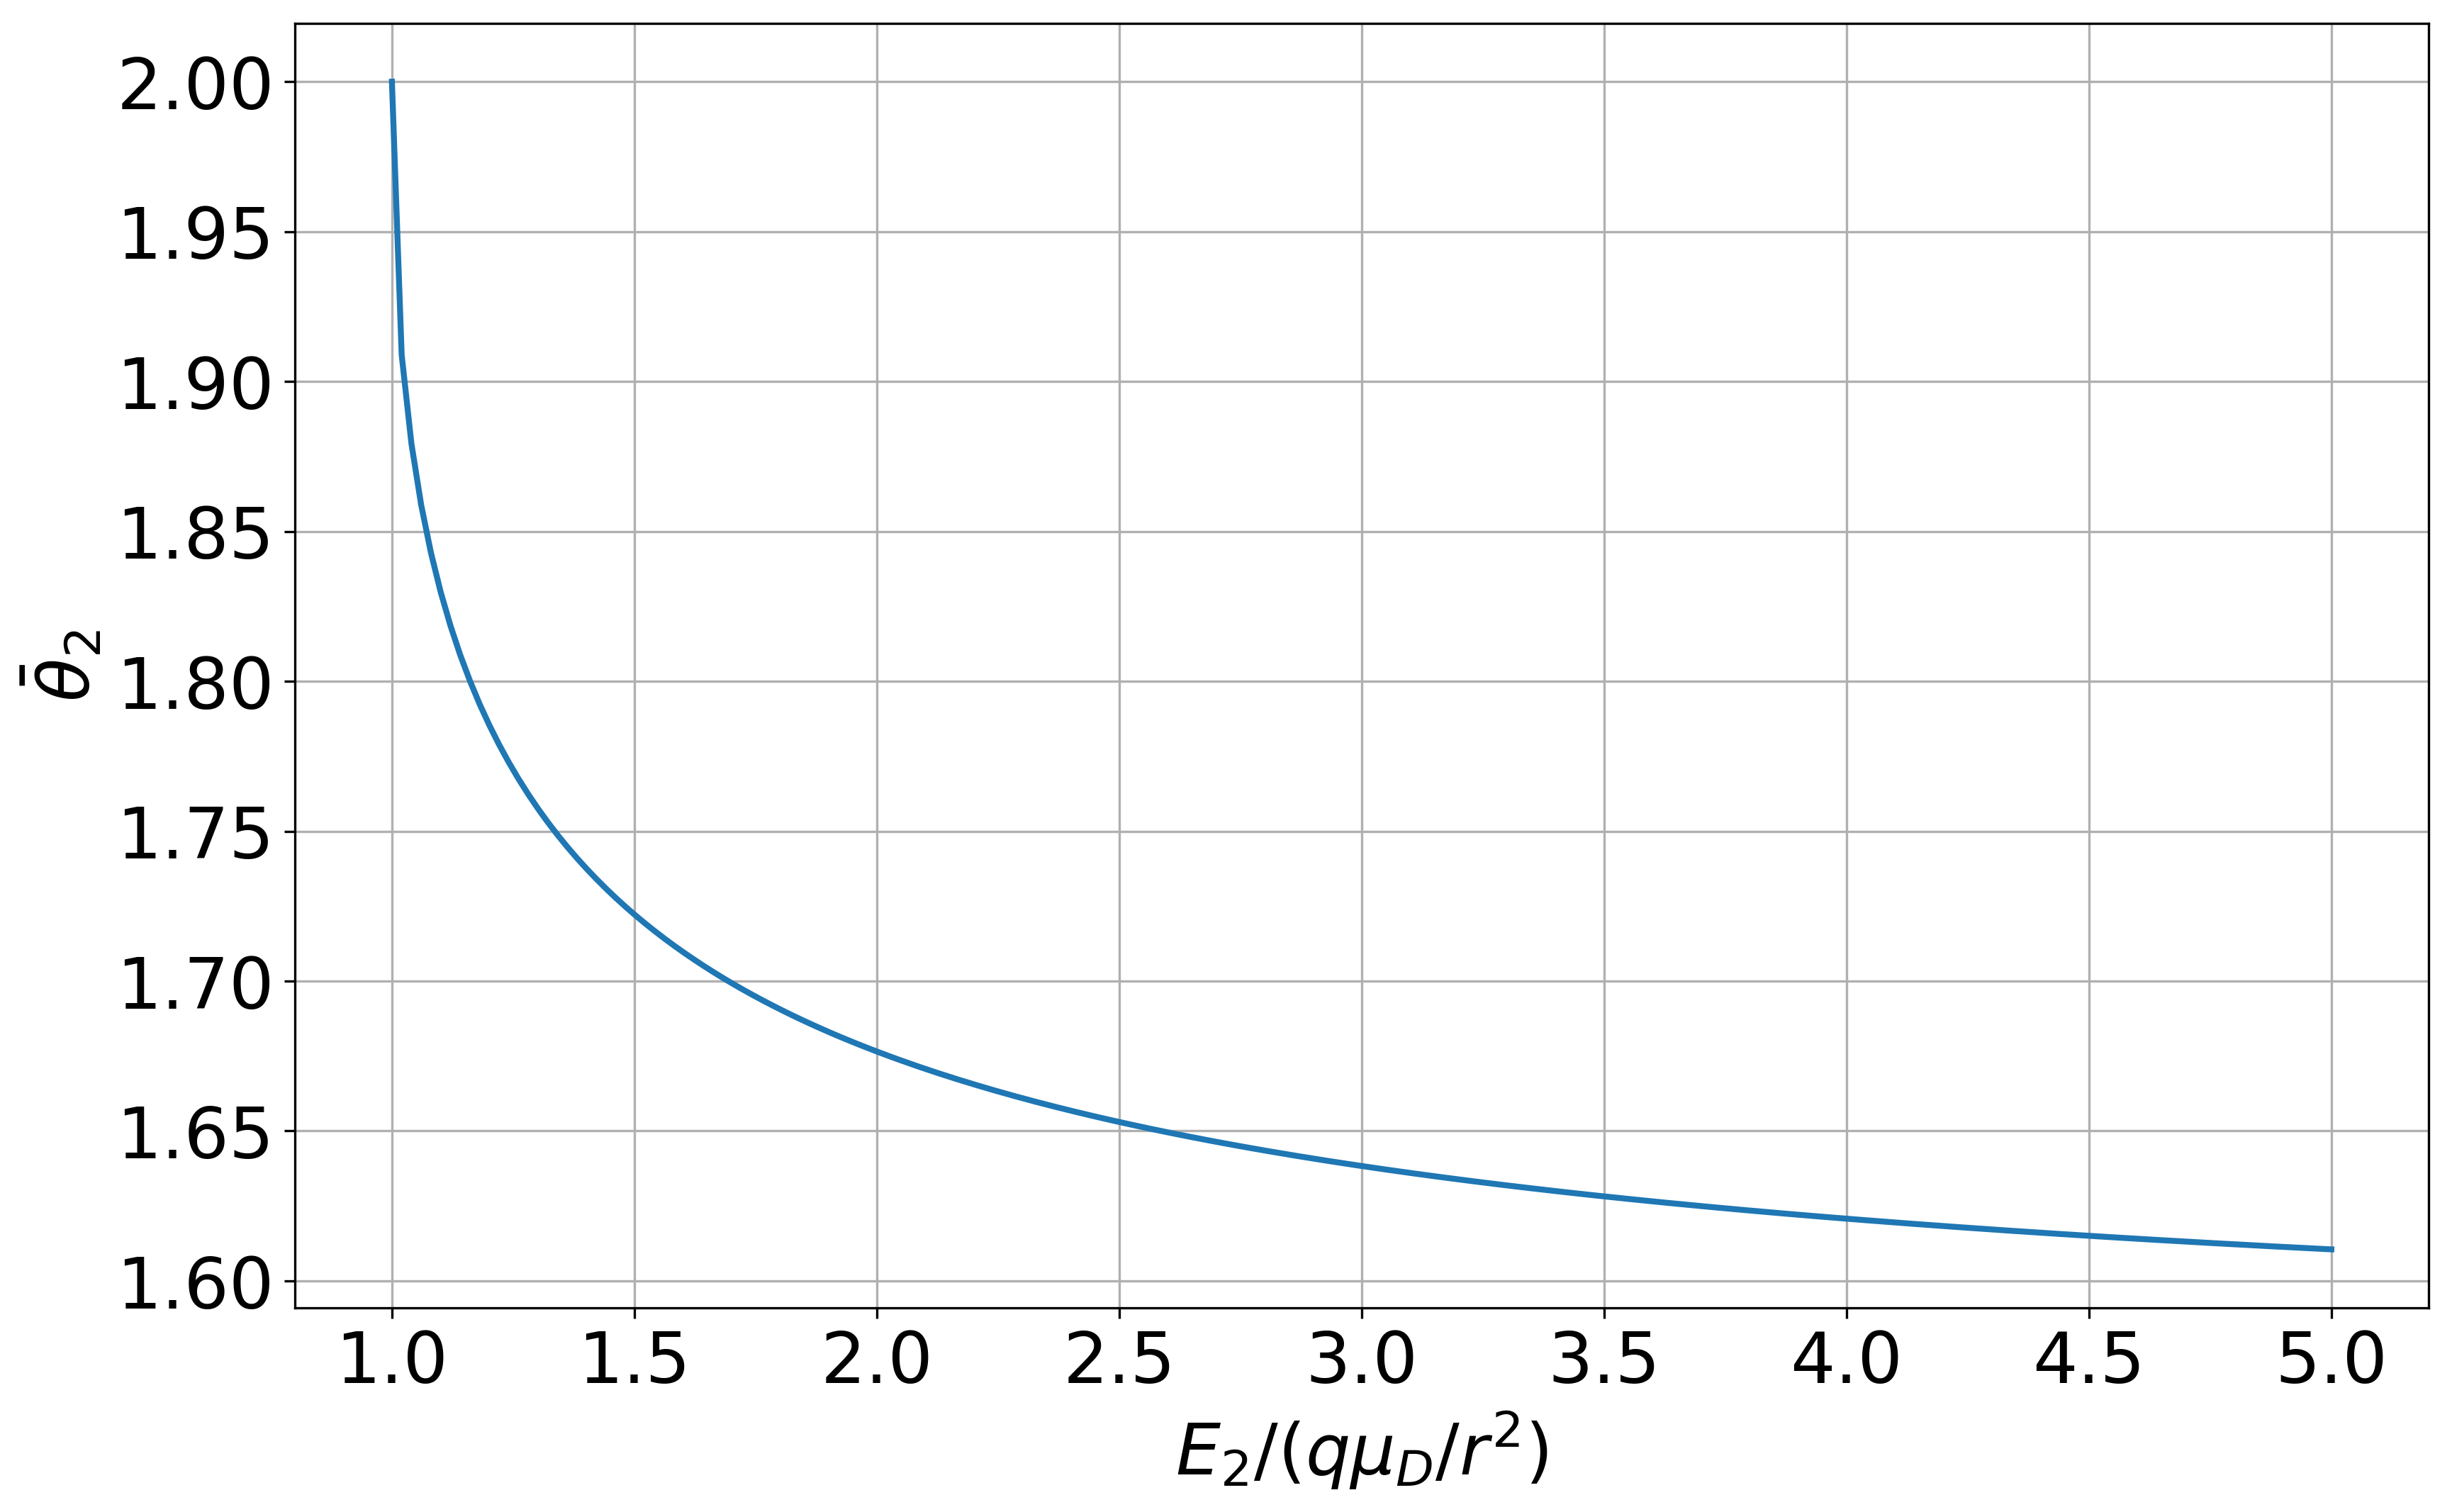
\includegraphics[width=0.8\textwidth]{images/ADO_theta2.png}
		\caption{Numerical solution to equation \ref{eq: theta2} as a function of the ratio of rotational energy and the monopole-dipole term. As the energy ratio increases, the more $\theta_2$ tends towards $\pi/2$.}
	\end{figure}

\end{enumerate}

Let's say we have the forms for $\bar{\theta_1}$ and $\bar{\theta_2}$, we want to write down the full form of $\theta$. We can combine the two weighted by the probability of each as a function of internal energy.

\begin{equation}
    \bar{\theta}(r) = \bar{\theta}_1(r) F_1 + \bar{\theta}_2(r) F_2 \label{eq: weighted theta}
\end{equation}

Where the weightings $F_i$ are found via:

\begin{equation*}
    P(\epsilon) d\epsilon = \frac{1}{k_BT}e^{-\frac{\epsilon}{k_BT}}d\epsilon
\end{equation*}

For diatomics, the energies of rotational states is defined as:
\begin{equation*}
    \epsilon = B_e J(J+1)
\end{equation*}

Where the rotational constant is $B_e=\frac{\hbar^2}{2\mu R^2}$, $\mu$ is the reduced mass of the molecule, and $R$ is the inter-nuclear separation. To find the rate constant, a similar process to that described in the general adiabatic capture theory derivation can be applied. A key assumption made to simplify the calculations is that the internal energy of the molecule and collision energy are in equilibrium, allowing us to integrate over one temperature distribution for equations \ref{eq: weighted theta} and \ref{eq: k(T)}. A parameterized form is given in Su et al. where the form is similar to that of just a Langevin term, but now with a dipole interaction term added onto it.\cite{Su1973}

\begin{equation}
    k_{ADO} = \frac{2 \pi e}{\sqrt{\mu}}\left(\sqrt{\alpha}+C \mu_D\sqrt{\frac{2}{\pi k_B T}}\right)
    \label{eq: k ADO}
\end{equation}

Where $C$ is the dipole locking constant. All of the terms aside from $C$ come from the integration over a Boltzmann distribution in $v$. $C$ itself can be numerically solved by iteratively integrating over combinations of $\mu_D$ and $\alpha$ shown in Figure \ref{fig: C}.\cite{Su1973}\cite{Troe1985}

\begin{figure}[H]
	\label{fig: C}
	\centering
	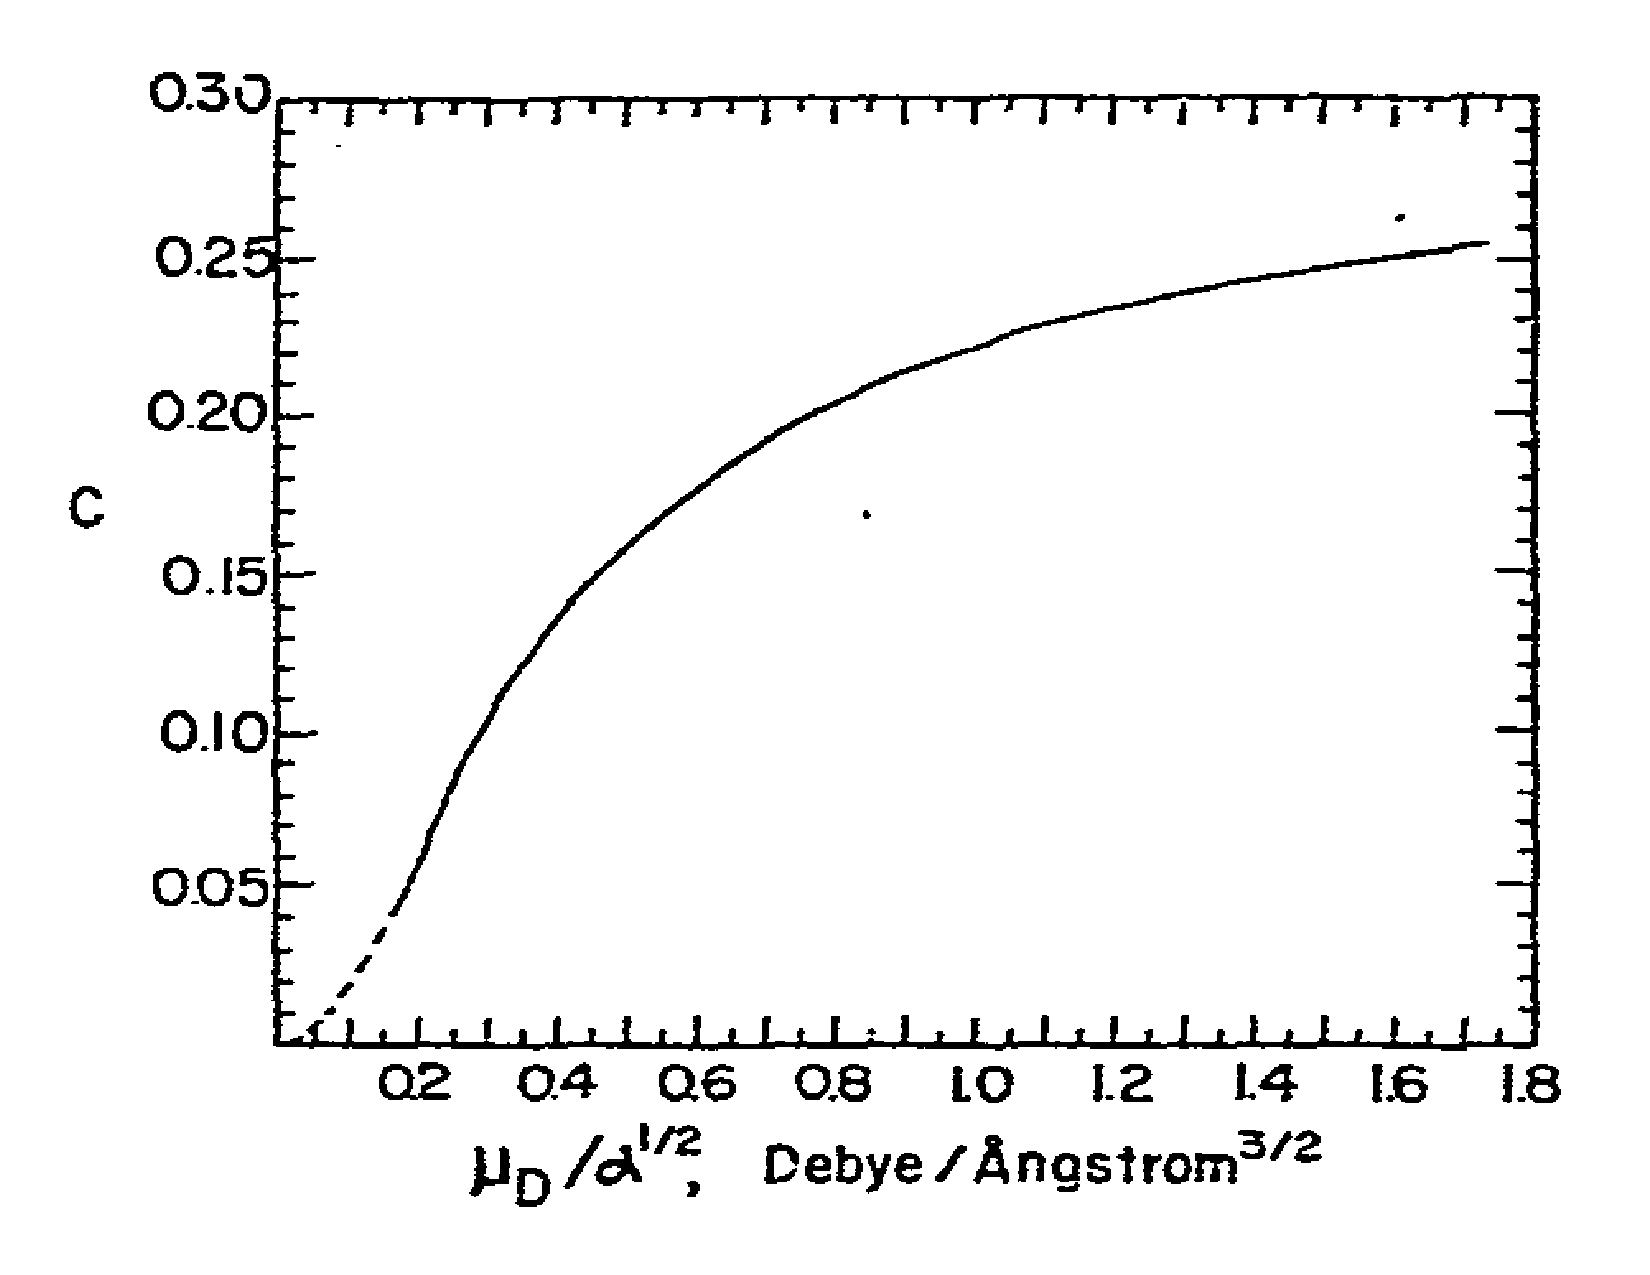
\includegraphics[width=0.8\textwidth]{images/ADO_C.pdf}
	\caption{Dipole locking constant $C$ parameterized by the dipole moment $\mu_D$ and polarizability $\alpha$.\cite{Su1973}}
\end{figure}
